\documentclass[conference]{IEEEtran}
% The preceding line is only needed to identify funding in the first footnote. If that is unneeded, please comment it out.
\usepackage{url,apacite}
\usepackage{amsmath,amssymb,amsfonts}
\usepackage{algorithmic}
\usepackage{graphicx}
\usepackage{textcomp}
\usepackage{xcolor}
\graphicspath{ {.} }
\bibliographystyle{apacite}
\def\BibTeX{{\rm B\kern-.05em{\sc i\kern-.025em b}\kern-.08em
T\kern-.1667em\lower.7ex\hbox{E}\kern-.125emX}}

\usepackage{listings}
\usepackage{xcolor}
 
\definecolor{codegreen}{rgb}{0,0.6,0}
\definecolor{codegray}{rgb}{0.5,0.5,0.5}
\definecolor{codepurple}{rgb}{0.58,0,0.82}
\definecolor{backcolour}{rgb}{0.95,0.95,0.92}

\lstdefinestyle{mystyle}{
    backgroundcolor=\color{backcolour},   
    commentstyle=\color{codegreen},
    keywordstyle=\color{magenta},
    numberstyle=\tiny\color{codegray},
    stringstyle=\color{codepurple},
    basicstyle=\ttfamily\footnotesize,
    breakatwhitespace=false,         
    breaklines=true,                 
    captionpos=b,                    
    keepspaces=true,                 
    numbers=left,                    
    numbersep=5pt,                  
    showspaces=false,                
    showstringspaces=false,
    showtabs=false,                  
    tabsize=2
}
     
\lstset{style=mystyle}

\begin{document}

\title{A microservices based approach for city traffic simulation}

\author{\IEEEauthorblockN{1\textsuperscript{st} Given Name Surname}
\IEEEauthorblockA{\textit{dept. name of organization (of Aff.)} \\
\textit{name of organization (of Aff.)}\\
City, Country \\
email address}
\and
\IEEEauthorblockN{2\textsuperscript{nd} Given Name Surname}
\IEEEauthorblockA{\textit{dept. name of organization (of Aff.)} \\
\textit{name of organization (of Aff.)}\\
City, Country \\
email address}
}

\maketitle

\begin{abstract}

Simulating traffic in a city is a difficult task. Current paper is proposing a novel way using state of the art in distributed systems: microservices orchestration. The design is centered around two types of actors: a city simulation actor (a single instance of it) which keeps track of occupied streets and and their gradual occupation. The other actor type (multiple instances) is the car which travels across the city.

\end{abstract}

\section{Introduction}

A solution which simulates car, pedestrian, etc. traffic in a given city may reap many benefits. It can help understand patterns of traffic and its flow. It can help unerstand the particularities and pecularities of a city's streets arrangements. It can help identify bottlenecks. It can help find solutions to rush problems and explore them. But for those areas to be tackled, appropiate methods of simulating traffic must be found. We are proposing a novel way of simulating traffic based on the microservices orchestration concept.

We define a \textbf{(city) actor} as being a independent entity which chose to move between two geographical points within a city. It can be a car, a pedestrian or a bike. We also define the \textbf{city simulator} as being a single entity (subject to distributed and load balacing services) which keeps data about the city (e.g. streets with city actors on them).

\section{Existing solutions}

(Summary of other papers with traffic simulation)

\section{Microservices}

\subsection{Current state}

Microservices are not a new concept. The idea behind them has existed since Linux kernel has started to be enriched with a concept called namespaces \cite{wiki:linuxns}. This allows one set of processes to see one set of resources while another set of processes see another set of resources, where resources might be, but not limited to, process IDs, file names and network resources. Those linux kernel abilities form the base of containers.

Thus, a container is a small set of processes which run in isolation. They allow packaging a linux distro, a set of libraries and skd and on top of those custom code. This forms an image, which is essentially a tar gzipped file. Once the build process of an image is finished, it can be spinned up in one or more running containers. The custom code written and embedded in the image is running in parallel in each container.

To go to solution for building, manipulating and running images is Docker \cite{docker}. It allows easy software installation, it works cross platform and it offers a smooth experience most of the time.

\section{Implementation}

The entities which are participating into a traffic simulation are called actors. They are two: the city actor and the city simulator. The supporting containers are not themselves part of traffic simulation but they do have an important and supporting role.

\subsection{City simulator}

The most common and easy solution to share data across all the city actors is to have a centralized store to keep it. City simulator acts as a centralized store for all other city actors. In the current implementation the city simulator keeps a set of data which can be described as a list of pairs, each pair having a line and a real number, called density.

The density is defined as the number of actors (cars) which are at a given moment present on a given segment of street. If the city simulator has no entry of a street segment then it will consider the density as being 0, i.e. there is no actor on that street. The density is modeled as an unsigned integer.

Figure \ref{fig:citysimrelations} depicts the city simulator in relation with the other entities. A notable exception is the web page. Its purpose is not to participate in the same information exchange the other have but to offer a visual interpretation of the way the city and the other actors are interacting with one another.

\begin{figure}
    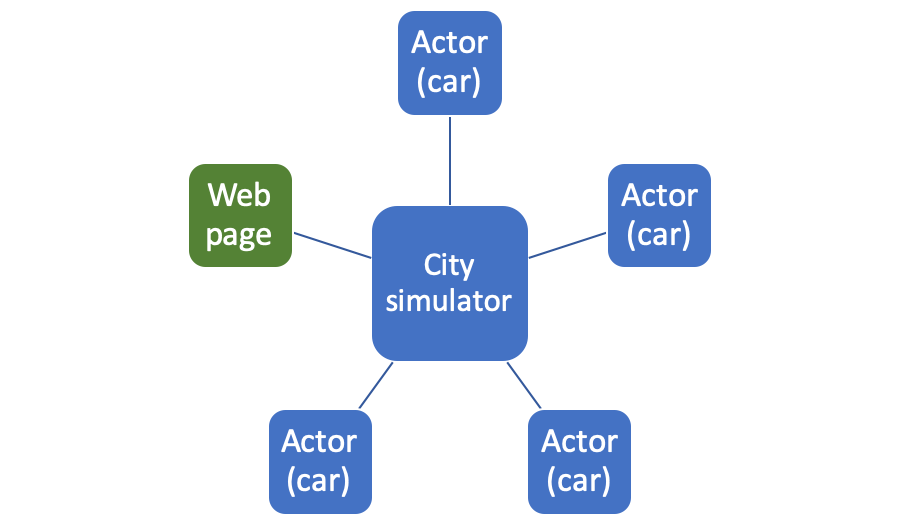
\includegraphics[width=8cm]{CitySimulator.png}
    \centering
    \caption{The relations of city simulator with other entities}
    \label{fig:citysimrelations}
\end{figure}

As various actors send data about their location, the city simulator needs to keep location and density data in its store. It does not know of Open Street Map maps and its corresponding map data sets but instead it requires any actor to send its current set of coordinates which it is crossing or which it left. If any other actor send the same set of coordinates, or a subset of it then the first set of coordinates will have its density incremented. Listing \ref{lst:goactorstruct} shows the Go struct which is used by an actor to send its report to the city simulator and is used by the city simulator to decode a message received from an actor. Apart from this line there are two more details to complete the report picture. Listing \ref{lst:goactorreports} contains the type of communications between actors and the citysimulator.

\begin{lstlisting}[caption=Go struct for actor's report, label=lst:goactorstruct]
// Report is the base type for reporting
// status and vectors to a city entity
type Report struct {
	CurrentLine  [][]float64
	ReportDetail int
}
\end{lstlisting}

As part of this proposal the city simulator is made to be a standalone entity (container) which communicates with actors. This might not be the case for other types of communications, as part of other architectures. One example can be the integration or the unifying of the city simulator with the city actor, both becoming one entity. In this case the communication between entities is subject to an entire panoply of choices.

\subsection{Car actor}

The city actor represents a moving actor within a city. It can be a car which moves across the city, it can be a bike or it can be a pedestrian. Its naming suggests that it can be any entity or living being which moves within a city and interacts with the other entities or affects the other entities in some manner. A pedestrian would directly interact with other pedestrians but not with cars. A pedestrian would indirectly affect other cars by willing to walk over a crossing.

The implementation proposed here is aiming to model a single type of actor: a car which moves between two points across a city. Because the purpose of this paper is not to tackle maps representation and routing through a city (in itself, this area is way bigger than a mere technical paper) the city actor is using two notable services: Open Street Map \cite{openstreetmap} and GraphHopper \cite{graphhopper}. Open Street Map is an open source licensed map of the entire world. Graphhoper is an open source service which offers directions APIs and route planning. It can use Open Street Map as an underlying map provider. They provider free tiers and paid subscription for accessing an API and get routes. However, a city actor is not using any public api but a special crafted container which contains GraphHopper and an open street map embedded into it. Thus, this container is running in parallel with the other city actors and provides them with the routing API they need.

A first way to introduce randomness into the entire simulation of a city is to choose a set of two coordinates inside the given city, a set for each city actor. Then the actor proceeds to ask GraphHopper service for a route between those two points. Because each city actor 'lives' only while its moving across its route and 'dies' as soon as it reached the finish point, the entire city simulation which takes place is made of independent, random and always new actors.

\subsection{Interactions}

An actor interacts, for the time being, with the city simulator by using a Go struct and a Go enum. They can be seen in listings \ref{lst:goactorstruct} and \ref{lst:goactorreports}.

\begin{lstlisting}[caption=Go struct for actor's report, label=lst:goactorreports]
const (   
    // ReportOnTheLine is the report sent by one agent to
    // notify the city that he is currently advancing
    // through one line.
    ReportOnTheLine = iota
    
    // ReportOffFromLine is the report sent by one agent to
    // notify the city that he has finished advancing through
    // one line and has departed from it.
    ReportOffFromLine = iota
)
    
const (
    // SendReport is a message passed from an actor to the city
    // indicating its status (e.g. location).
    SendReport = iota
    
    // AskForLine is a message passed from an actor to the city.
    // A response is awaited.
    AskForLine = iota
    
    // RespondWithLine is a message passed from the city to
    // an actor and it contains line data.
    RespondWithLine = iota
)
\end{lstlisting}

\section{Orchestration}

\subsection{Current state}

\subsection{Implementation}

\subsection{Docker compose}

\subsection{Kubernetes}

\section{Design choices}

\subsection{Tools and programming languages}
\begin{itemize}
\item Go programming language
\item Docker
\item Docker compose
\item Web page choices (web page will become an actor)
\end{itemize}

\subsection{Choices and rationales}

\subsection{Alternatives}
(Actor model and consacrated frameworks)

\subsection{Networking design}

\subsection{Orchestration design}

\section{Results}

\subsection{Visual}

\subsection{Performance}

\section{Enhancements}
(Distributed database for multiple city simulators)

(More granular logic on actor behavior)

(More types of "junctions": classic junction for cars, pedestrian crossings, subways access stairs and elevators, bus stations, etc.)

(Contained actors: pedestrians in a bus, pedestrian in a subway)

\bibliography{wiki}
\vspace{12pt}

\end{document}
